% =============================================================================
% SchemaForge v2.0 -- Implementation Plan
% Build (MiKTeX):  pdflatex SchemaForge_Implementation_Plan.tex   (run twice)
%            or:  latexmk -pdf SchemaForge_Implementation_Plan.tex
% =============================================================================
\documentclass[11pt,a4paper]{article}

% ---------- Encoding & fonts ----------
\usepackage[T1]{fontenc}
\usepackage[utf8]{inputenc}
\usepackage{lmodern}
\usepackage[scaled=0.92]{helvet}
\usepackage{microtype}

% ---------- Layout ----------
\usepackage[margin=2.2cm,headheight=15pt]{geometry}
\usepackage{fancyhdr}
\usepackage{titlesec}
\usepackage{enumitem}
\usepackage{parskip}

% ---------- Tables, colour, graphics ----------
\usepackage{xcolor}  % no [table]: MiKTeX's colortbl 2024 is newer than its array 2023 and breaks p-columns
\usepackage{array,booktabs,tabularx,longtable,multirow}
\usepackage{tikz}
\usetikzlibrary{positioning,arrows.meta,fit,backgrounds,shapes.geometric,calc}
\usepackage[skins,breakable]{tcolorbox}
\usepackage{listings}
\usepackage{amssymb}

% ---------- Links (load late) ----------
\usepackage[hidelinks]{hyperref}
\usepackage{xurl}  % lets long identifiers break at any character
\urlstyle{tt}
\makeatletter
\g@addto@macro{\UrlBreaks}{\do\/\do\_\do-\do.}
\makeatother

% ---------- Palette ----------
\definecolor{sfnavy}{HTML}{1B2A41}
\definecolor{sfblue}{HTML}{2F5D8A}
\definecolor{sfteal}{HTML}{2A8C82}
\definecolor{sfgrey}{HTML}{5B6573}
\definecolor{sflight}{HTML}{EEF2F6}
\definecolor{sfred}{HTML}{B3261E}
\definecolor{sforange}{HTML}{C0661A}
\definecolor{sfamber}{HTML}{9A7B00}
\definecolor{sfgreen}{HTML}{2E7D32}
\definecolor{codebg}{HTML}{F6F8FA}

% ---------- Headings ----------
\titleformat{\section}{\sffamily\Large\bfseries\color{sfnavy}}{\thesection}{0.8em}{}[{\color{sfblue}\titlerule[0.8pt]}]
\titleformat{\subsection}{\sffamily\large\bfseries\color{sfblue}}{\thesubsection}{0.7em}{}
\titleformat{\subsubsection}{\sffamily\normalsize\bfseries\color{sfnavy}}{\thesubsubsection}{0.6em}{}
\titlespacing*{\section}{0pt}{1.6em}{0.8em}

% ---------- Header / footer ----------
\pagestyle{fancy}
\fancyhf{}
\fancyhead[L]{\sffamily\small\color{sfgrey}SchemaForge v2.0}
\fancyhead[R]{\sffamily\small\color{sfgrey}Implementation Plan}
\fancyfoot[C]{\sffamily\small\color{sfgrey}\thepage}
\renewcommand{\headrulewidth}{0.4pt}

% ---------- Macros ----------
\newcommand{\fp}[1]{\nolinkurl{#1}}  % file paths / identifiers (no spaces)
\newcommand{\sev}[2]{\colorbox{#1}{\textcolor{white}{\sffamily\scriptsize\bfseries\strut #2}}}
\newcommand{\crit}{\sev{sfred}{CRITICAL}}
\newcommand{\high}{\sev{sforange}{HIGH}}
\newcommand{\med}{\sev{sfamber}{MEDIUM}}
\newcommand{\low}{\sev{sfgrey}{LOW}}
\newcommand{\done}{\textcolor{sfgreen}{\ensuremath{\checkmark}}}
\newcommand{\wip}{\textcolor{sfamber}{\ensuremath{\sim}}}
\newcommand{\missing}{\textcolor{sfred}{\ensuremath{\times}}}
\newcolumntype{L}[1]{>{\raggedright\arraybackslash}p{#1}}
\newcolumntype{Y}{>{\raggedright\arraybackslash}X}
\setlist{itemsep=2pt,topsep=4pt}
\renewcommand{\arraystretch}{1.25}
\setlength{\emergencystretch}{3em}

% ---------- Boxes ----------
\newtcolorbox{keybox}[1]{enhanced,breakable,colback=sflight,colframe=sfblue,
  boxrule=0pt,leftrule=3pt,arc=0pt,left=8pt,right=8pt,top=6pt,bottom=6pt,
  fonttitle=\sffamily\bfseries,coltitle=sfnavy,
  title={#1},attach title to upper={\par\smallskip}}
\newtcolorbox{warnbox}[1]{enhanced,breakable,colback=sfred!5,colframe=sfred,
  boxrule=0pt,leftrule=3pt,arc=0pt,left=8pt,right=8pt,top=6pt,bottom=6pt,
  fonttitle=\sffamily\bfseries,coltitle=sfred,
  title={#1},attach title to upper={\par\smallskip}}
\newtcolorbox{acceptbox}{enhanced,breakable,colback=sfgreen!5,colframe=sfgreen,
  boxrule=0pt,leftrule=3pt,arc=0pt,left=8pt,right=8pt,top=6pt,bottom=6pt,
  fonttitle=\sffamily\bfseries,coltitle=sfgreen,
  title={Acceptance criteria},attach title to upper={\par\smallskip}}

% ---------- Code listings ----------
\lstdefinelanguage{TypeScript}{
  keywords={async,await,const,let,function,return,if,else,throw,try,catch,finally,
    interface,type,export,import,from,new,for,of,in,class,private,public,true,false,null,undefined},
  morecomment=[l]{//}, morecomment=[s]{/*}{*/},
  morestring=[b]', morestring=[b]",
  sensitive=true}
\lstset{
  basicstyle=\ttfamily\footnotesize,
  backgroundcolor=\color{codebg},
  keywordstyle=\color{sfblue}\bfseries,
  commentstyle=\color{sfgrey}\itshape,
  stringstyle=\color{sfteal},
  frame=l, framerule=2pt, rulecolor=\color{sfblue!40},
  xleftmargin=10pt, framexleftmargin=6pt,
  breaklines=true, columns=fullflexible, keepspaces=true,
  showstringspaces=false, tabsize=2,
  upquote=true,
  aboveskip=8pt, belowskip=8pt}

\hypersetup{pdftitle={SchemaForge v2.0 Implementation Plan},pdfauthor={SchemaForge Team}}

% =============================================================================
\begin{document}

% ------------------------------ Title page ----------------------------------
\begin{titlepage}
\begin{tikzpicture}[remember picture,overlay]
  \fill[sfnavy] (current page.north west) rectangle ([yshift=-9.5cm]current page.north east);
  \fill[sfteal] ([yshift=-9.5cm]current page.north west) rectangle ([yshift=-9.8cm]current page.north east);
  \node[anchor=north west,text=white,font=\sffamily,align=left,text width=16cm]
    at ([xshift=2.2cm,yshift=-2.4cm]current page.north west)
    {{\large\color{sfteal!50!white} TrueFoundry $\times$ Polaris \quad ``Agents That Act''}\\[1.2cm]
     {\fontsize{34}{38}\selectfont\bfseries SchemaForge v2.0}\\[0.4cm]
     {\LARGE Implementation Plan}\\[0.5cm]
     {\large Autonomous Database Migration Reliability Agent}};
\end{tikzpicture}

\vspace*{8.6cm}

{\sffamily\large\color{sfnavy}
From the current repository to a judge-ready, evidence-backed migration agent with a
hard production approval boundary.}

\vspace{1.2cm}

\begin{tabularx}{\textwidth}{@{}L{4.2cm}Y@{}}
\toprule
\sffamily\bfseries Document & Engineering implementation plan \\
\sffamily\bfseries Baseline & Repository state as of 26 September 2026 and \fp{SchemaForge_v2_Engineering_Playbook.pdf} \\
\sffamily\bfseries Stack & TrueForge, MCP (TypeScript, \fp{@modelcontextprotocol/sdk}), PostgreSQL 16, Docker Compose \\
\sffamily\bfseries Scope & PostgreSQL only; one e-commerce schema; one failing and one safe scenario \\
\sffamily\bfseries Estimated effort & About 7.5 focused engineering hours across 6 phases \\
\bottomrule
\end{tabularx}

\vfill
\begin{keybox}{Guiding principle}
The agent may reason and rehearse autonomously. Production mutation is a separate,
action-bound, human-authorised capability that the agent process cannot forge,
reuse, or apply to a schema that has drifted.
\end{keybox}
\end{titlepage}

\tableofcontents
\newpage

% =============================================================================
\section{Objective and Definition of Done}

SchemaForge turns a natural-language migration request into an evidence-backed
decision. The repository already contains a skeleton of every component described in
the playbook. This plan closes the gap between that skeleton and a system whose safety
claims are enforced by code and by the database, not only by documentation.

\begin{keybox}{Definition of done (from the playbook, made testable)}
\begin{enumerate}[leftmargin=*]
  \item A TrueForge session inspects the real PostgreSQL target through the read-only role.
  \item Request A (\emph{``make \fp{users.email} NOT NULL''}) is rehearsed on an isolated
        copy of representative data, the 14 seeded NULL emails are found, and the
        deterministic decision engine returns \textbf{DO NOT APPLY}. Production is untouched.
  \item Request B (\emph{``add a nullable \fp{archived_at} column to users''}) passes all checks, TrueForge
        freezes, a human mints a signed approval bound to that exact SQL and schema
        fingerprint, and the separate executor applies it.
  \item Read-only post-apply verification confirms the new column and unchanged invariants.
  \item Replaying the same approval, editing the SQL, or changing the schema before apply
        is rejected, and each rejection is covered by an automated test.
\end{enumerate}
\end{keybox}

% =============================================================================
\section{Current State Assessment}

\subsection{Component inventory}

The MCP server type-checks cleanly (\texttt{tsc -{}-noEmit} reports no errors). The table
records whether each playbook capability works end to end.

\begin{longtable}{@{}L{4.1cm}L{5.4cm}c L{4.6cm}@{}}
\toprule
\sffamily\bfseries Capability & \sffamily\bfseries Location & \sffamily\bfseries State & \sffamily\bfseries Note \\
\midrule
\endhead
Two PostgreSQL 16 containers & \fp{docker-compose.yml} & \done & prod :5433, shadow :5434 \\
Read-only role \fp{sf_reader} & \fp{docker/init-prod.sql} & \done & SELECT grants and default privileges \\
Schema inspection and fingerprint & \fp{mcp-server/src/tools/inspect_schema.ts} & \done & row counts are \fp{reltuples} estimates \\
Read-only query tool & \fp{mcp-server/src/tools/readonly_query.ts} & \wip & regex and row cap; no read-only transaction \\
Dependency analysis & \fp{mcp-server/src/tools/analyze_dependencies.ts} & \wip & database objects only, no repository scan \\
Shadow rehearsal & \fp{mcp-server/src/tools/rehearse_migration.ts} & \wip & not isolated; transaction bug (F2) \\
Gated executor & \fp{mcp-server/src/tools/execute_migration.ts} & \wip & unsigned token, no drift check \\
Post-apply verification & \fp{mcp-server/src/tools/verify_production.ts} & \done & table name interpolated (F12) \\
Seeded edge cases & \fp{shadow/seed-edge-cases.sql} & \done & 14 NULL emails, 3 duplicates, and more \\
Invariant and fingerprint library & \fp{verification/*.ts} & \wip & not wired into the server \\
Execution-mode classifier & \fp{types.ts} (\fp{MigrationClassification}) & \missing & type exists, unused \\
Decision engine & \fp{types.ts} (\fp{DecisionPacket}) & \missing & type exists, unused \\
Approval minting and ledger & --- & \missing & nothing issues or consumes tokens \\
Automated tests & --- & \missing & none in repository \\
\bottomrule
\end{longtable}

{\small Legend: \done{} implemented \quad \wip{} partial \quad \missing{} absent}

\subsection{Findings}

Each finding was confirmed by reading the referenced file. Severity reflects impact on
the definition of done: \crit{} blocks the demo or voids a safety claim,
\high{} weakens a safety claim, \med{} and \low{} affect quality or honesty of evidence.

\begin{longtable}{@{}L{0.7cm}L{1.8cm}L{6.9cm}L{5.2cm}@{}}
\toprule
\sffamily\bfseries ID & \sffamily\bfseries Severity & \sffamily\bfseries Finding & \sffamily\bfseries Evidence \\
\midrule
\endhead
F1 & \crit & Environment variable names disagree. The server reads
  \fp{SF_PROD_READONLY_URL}, \fp{SF_PROD_WRITE_URL} and \fp{SF_SHADOW_URL}; \fp{.env.example} and
  \fp{agent.yaml} provide \fp{PROD_READONLY_URL}, \fp{PROD_DATABASE_URL} and \fp{SHADOW_DATABASE_URL}.
  No pool is created, so every tool call fails. & \fp{mcp-server/src/db.ts} lines 38--71;
  \fp{trueforge-config/agent.yaml} \\
F2 & \crit & Transactions span different connections. \fp{db.query()} checks out a fresh
  pooled client per call, so \texttt{BEGIN}, the migration and \texttt{COMMIT} run in separate
  sessions. \texttt{ROLLBACK} does nothing, and a failed multi-statement migration can be half applied.
  & \fp{db.ts} \fp{query()}; \fp{rehearse_migration.ts}; \fp{execute_migration.ts} \\
F3 & \crit & Demo data is not where the demo needs it. Production is created with
  \texttt{email NOT NULL} and zero rows, and the shadow init mirrors that strict schema. The nullable
  schema and 14 NULL emails exist only in \fp{shadow/seed-*.sql}, which Compose never loads.
  Request A is already satisfied in production and rehearses with no violations.
  & \fp{docker/init-prod.sql}, \fp{docker/init-shadow.sql}, \fp{shadow/seed-schema.sql} \\
F4 & \high & The reset script authenticates as \texttt{postgres/postgres}; the shadow container's
  superuser is \fp{sf_shadow}. & \fp{shadow/reset-shadow.sh} \\
F5 & \crit & Approval tokens are unsigned and supplied by the caller, including the
  \fp{used} flag. The agent can fabricate a valid token for any SQL, and single use is
  not enforced server-side. & \fp{execute_migration.ts} checks 1--4; \fp{ApprovalToken} in \fp{types.ts} \\
F6 & \crit & The pre-apply schema drift check is described in the header comment but not
  implemented, and the token carries no fingerprint. & \fp{execute_migration.ts} lines 14--17 \\
F7 & \high & No statement classifier. Tier-3 prohibitions exist only in YAML, and every
  migration is wrapped in \texttt{BEGIN}, so \texttt{CREATE INDEX CONCURRENTLY} fails.
  & \fp{MigrationClassification} unused \\
F8 & \high & The production write pool lives in the same process as the agent's
  read and rehearsal tools, which contradicts the playbook's credential rule. & \fp{prodWrite} pool in \fp{db.ts} \\
F9 & \high & Rehearsal commits into one long-lived shadow database, so each run mutates the
  baseline for the next. Evidence is not deterministic. & \fp{rehearse_migration.ts} \\
F10 & \med & \fp{verification/} is a separate package without installed dependencies and is
  not imported; fingerprinting is implemented twice. & \fp{verification/package.json}; \fp{inspect_schema.ts} \\
F11 & \med & No deterministic decision engine; APPLY, REVIEW or DO NOT APPLY is left to the LLM. & \fp{DecisionPacket} unused \\
F12 & \med & \fp{table_name} is interpolated directly into SQL. & smoke test in \fp{verify_production.ts} \\
F13 & \med & The read-only tool relies on regex plus role grants; sessions are not forced read-only. & \fp{readonly_query.ts} \\
F14 & \low & Row counts come from \fp{pg_class.reltuples} and must be flagged as estimates. & \fp{inspect_schema.ts} line 80 \\
F15 & \low & The README describes \fp{src/server.ts}, HTTP port 3100 and a root \texttt{npm install};
  the real server is \fp{mcp-server/} on stdio. & \fp{README.md} \\
F16 & \med & No automated tests for any safety property. & repository \\
\bottomrule
\end{longtable}

\begin{warnbox}{Honest evidence note}
The playbook's sample packet quotes 182{,}340 rows inspected. The seed currently creates
500 users. Either scale the seed (Phase~2) or show the real number. The
packet must never display a figure that was not measured.
\end{warnbox}

% =============================================================================
\section{Target Architecture}

The main change is splitting the MCP layer into two processes with different
credentials, and moving approval minting to a human-side tool whose signing secret the
agent never sees.

\begin{center}
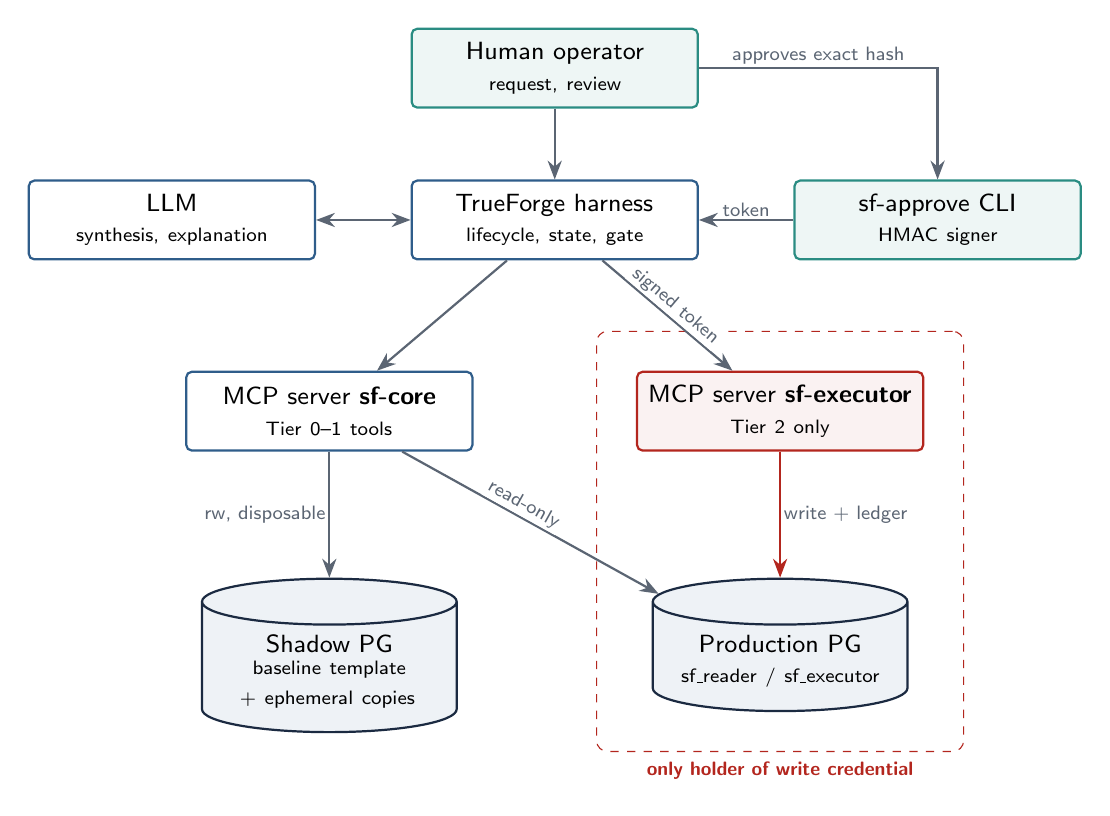
\begin{tikzpicture}[
  font=\sffamily\small, node distance=9mm and 12mm,
  box/.style={draw=sfblue,fill=white,rounded corners=2pt,thick,align=center,
              minimum height=10mm,text width=34mm},
  hum/.style={box,draw=sfteal,fill=sfteal!8},
  db/.style={cylinder,shape border rotate=90,aspect=0.18,draw=sfnavy,fill=sflight,
             thick,align=center,minimum height=16mm,text width=30mm},
  gate/.style={box,draw=sfred,fill=sfred!6},
  arr/.style={-{Stealth[length=2.4mm]},thick,sfgrey},
  lbl/.style={font=\sffamily\scriptsize,text=sfgrey,fill=white,inner sep=1pt}]

  \node[hum] (human) {Human operator\\\scriptsize request, review};
  \node[box,below=of human] (tf) {TrueForge harness\\\scriptsize lifecycle, state, gate};
  \node[box,left=of tf] (model) {LLM\\\scriptsize synthesis, explanation};
  \node[hum,right=of tf] (approve) {sf-approve CLI\\\scriptsize HMAC signer};
  \node[box,below left=14mm and -8mm of tf] (core) {MCP server \textbf{sf-core}\\\scriptsize Tier 0--1 tools};
  \node[gate,below right=14mm and -8mm of tf] (exec) {MCP server \textbf{sf-executor}\\\scriptsize Tier 2 only};

  \node[db,below=16mm of core] (shadow) {Shadow PG\\\scriptsize baseline template\\\scriptsize + ephemeral copies};
  \node[db,below=16mm of exec] (prod) {Production PG\\\scriptsize sf\_reader / sf\_executor};

  \draw[arr] (human) -- (tf);
  \draw[{Stealth[length=2.4mm]}-{Stealth[length=2.4mm]},thick,sfgrey] (model) -- (tf);
  \draw[arr] (human) -| node[lbl,pos=0.25,above]{approves exact hash} (approve);
  \draw[arr] (approve) -- node[lbl,above]{token} (tf);
  \draw[arr] (tf) -- (core);
  \draw[arr] (tf) -- node[lbl,sloped,above]{signed token} (exec);
  \draw[arr] (core) -- node[lbl,left]{rw, disposable} (shadow);
  \draw[arr] (core) -- node[lbl,sloped,above,pos=0.45]{read-only} (prod);
  \draw[arr,sfred] (exec) -- node[lbl,right]{write + ledger} (prod);

  \begin{scope}[on background layer]
    \node[draw=sfred,dashed,rounded corners,fit=(exec)(prod),inner sep=5mm,
          label={[font=\sffamily\scriptsize\bfseries,text=sfred]south:only holder of write credential}] {};
  \end{scope}
\end{tikzpicture}
\end{center}

\subsection{Trust boundaries}
\begin{itemize}[leftmargin=*]
  \item \textbf{sf-core} holds \fp{SF_PROD_READONLY_URL} and \fp{SF_SHADOW_URL} only. Its tools are
        \fp{db_inspect_schema}, \fp{db_run_readonly_query}, \fp{analyze_dependencies},
        \fp{rehearse_migration}, \fp{build_decision_packet} and \fp{verify_production}.
  \item \textbf{sf-executor} holds \fp{SF_PROD_WRITE_URL} and \fp{SF_APPROVAL_SECRET}
        and exposes one tool, \fp{execute_migration}.
  \item \textbf{sf-approve} runs in the human's terminal, displays the decision packet,
        requires typing the migration hash prefix, and signs. The default answer is reject.
  \item Production write access uses a dedicated \fp{sf_executor} role (DDL on
        \fp{public}, INSERT on the ledger), not the container superuser \fp{sf_admin}.
\end{itemize}

% =============================================================================
\section{Implementation Phases}

Each phase lists tasks, touched files and acceptance criteria. Phases 0 and 1 are
mandatory before any demo rehearsal, and everything later builds on them.

% -----------------------------------------------------------------------------
\subsection{Phase 0: Unblock the pipeline (1.5 h)}
\label{sec:p0}

\begin{enumerate}[leftmargin=*,label=\textbf{0.\arabic*}]
  \item \textbf{Single validated config} (F1). Add \fp{mcp-server/src/config.ts}, which parses
        \fp{process.env} with \fp{zod}, uses one naming scheme (\fp{SF_*}), and fails fast
        with a clear message. Update \fp{.env.example} and \fp{agent.yaml} to match.
  \item \textbf{Connection-scoped transactions} (F2). Add \fp{withClient} and
        \fp{withTransaction} to \fp{DatabaseManager}, and remove every bare
        \texttt{BEGIN}/\texttt{COMMIT} issued through \fp{db.query()}. Use \texttt{SET LOCAL} for timeouts.
  \item \textbf{Align demo data} (F3). Production represents the real target, so it
        must hold the nullable schema and representative rows. Load \fp{shadow/seed-schema.sql},
        \fp{seed-data.sql} and \fp{seed-edge-cases.sql} into prod through Compose init scripts
        (prefixes \fp{02-}, \fp{03-}, \fp{04-}), then apply role grants. Shadow is populated
        from prod (Phase 2), not from its own schema file.
  \item \textbf{Fix the reset script} (F4). Default to \fp{sf_shadow} credentials read from \fp{.env}.
  \item \textbf{README truth pass} (F15). Correct paths, transport and install steps.
\end{enumerate}

\begin{lstlisting}[language=TypeScript]
// db.ts -- every multi-statement unit of work runs on ONE session
async withTransaction<T>(
  pool: PoolName,
  fn: (client: pg.PoolClient) => Promise<T>,
  opts: { timeoutMs?: number; readOnly?: boolean } = {},
): Promise<T> {
  const client = await this.getPool(pool).connect();
  try {
    await client.query(opts.readOnly ? 'BEGIN READ ONLY' : 'BEGIN');
    const ms = Math.trunc(opts.timeoutMs ?? this.statementTimeoutMs);
    await client.query(`SET LOCAL statement_timeout = ${ms}`);
    const result = await fn(client);
    await client.query('COMMIT');
    return result;
  } catch (err) {
    await client.query('ROLLBACK').catch(() => {});
    throw err;
  } finally {
    client.release();
  }
}
\end{lstlisting}

\begin{acceptbox}
\begin{itemize}[leftmargin=*]
  \item \texttt{docker compose down -v \&\& docker compose up -d} yields prod with 500 or more users
        and exactly 14 NULL emails.
  \item The server starts with the \fp{.env.example} values and all tools connect.
  \item The test migration \texttt{ALTER TABLE users ADD COLUMN x int; SELECT 1/0;} leaves no
        column \texttt{x} behind.
\end{itemize}
\end{acceptbox}

% -----------------------------------------------------------------------------
\subsection{Phase 1: Safety core (2 h)}
\label{sec:p1}

\subsubsection*{1.1 Statement classifier (F7)}
Create \fp{mcp-server/src/safety/classifier.ts}. Parse with a real SQL parser
(\fp{pgsql-ast-parser}, exact pinned version) rather than regex, split multi-statement
input, and classify each statement. \textbf{Fail closed}: anything unparseable is
PROHIBITED for execution and REVIEW for the decision.

\begin{longtable}{@{}L{6.2cm}L{3.8cm}L{5.0cm}@{}}
\toprule
\sffamily\bfseries Statement pattern & \sffamily\bfseries Class & \sffamily\bfseries Execution mode \\
\midrule
\texttt{ADD COLUMN} (nullable, no volatile default) & TRANSACTIONAL & single transaction with \fp{lock_timeout} \\
\texttt{SET NOT NULL}, \texttt{ADD CONSTRAINT} & TRANSACTIONAL & validate first (see Phase 2) \\
\texttt{CREATE/DROP INDEX CONCURRENTLY}, \texttt{REINDEX CONCURRENTLY} & NON\_\allowbreak TRANSACTIONAL & autocommit, one statement per call \\
\texttt{DROP TABLE}, \texttt{TRUNCATE}, \texttt{DROP DATABASE}, \texttt{DROP SCHEMA} & PROHIBITED & rejected at every layer \\
\texttt{GRANT}, \texttt{REVOKE}, \texttt{ALTER ROLE}, \texttt{CREATE ROLE} & PROHIBITED & rejected at every layer \\
\texttt{DELETE}/\texttt{UPDATE} without \texttt{WHERE}, \texttt{DROP COLUMN} & PROHIBITED & escalated, not executable \\
Mixed transactional and non-transactional & PROHIBITED & must be split into separate migrations \\
\bottomrule
\end{longtable}

The classifier runs in \fp{rehearse_migration} and \fp{build_decision_packet}, and again inside
\fp{execute_migration}. The \fp{sf_executor} role has no \texttt{TRUNCATE}, no role
management, and does not own tables it must not drop, so the database remains a boundary
even if the classifier is wrong.

\subsubsection*{1.2 Signed, action-bound approvals (F5, F6)}

\begin{lstlisting}[language=TypeScript]
// safety/approval.ts -- shared by sf-approve (sign) and sf-executor (verify)
export interface ApprovalPayload {
  migration_hash: string;      // sha256 of normalised SQL
  target: 'prod';
  schema_fingerprint: string;  // fingerprint captured at rehearsal time
  action: string;              // human-readable summary shown at approval
  nonce: string;               // crypto.randomUUID()
  issued_at: string;
  expires_at: string;          // issued_at + SF_APPROVAL_TTL_SECONDS
}
export interface SignedApproval { payload: ApprovalPayload; sig: string }

export function sign(p: ApprovalPayload, secret: Buffer): SignedApproval {
  const sig = createHmac('sha256', secret).update(canonicalJson(p)).digest('hex');
  return { payload: p, sig };
}

export function verify(a: SignedApproval, secret: Buffer): boolean {
  const expected = createHmac('sha256', secret)
    .update(canonicalJson(a.payload)).digest();
  const given = Buffer.from(a.sig, 'hex');
  return given.length === expected.length && timingSafeEqual(given, expected);
}
\end{lstlisting}

The \fp{used} field is removed from the token. Single use is enforced by a ledger in
production, written in the same transaction as the migration:

\begin{lstlisting}[language=SQL]
CREATE SCHEMA sf_audit;
CREATE TABLE sf_audit.consumed_approvals (
  nonce          uuid        PRIMARY KEY,
  migration_hash text        NOT NULL,
  fingerprint    text        NOT NULL,
  consumed_at    timestamptz NOT NULL DEFAULT now(),
  outcome        text        NOT NULL
);
\end{lstlisting}

\subsubsection*{1.3 Executor sequence}
\begin{enumerate}[leftmargin=*,label=\arabic*.]
  \item Verify the HMAC signature, expiry and \fp{target}.
  \item Recompute \fp{sha256} of the normalised SQL; it must equal \fp{migration_hash}.
  \item Re-classify and reject anything PROHIBITED.
  \item Recapture the schema fingerprint through \fp{sf_reader}. A mismatch returns
        \fp{SCHEMA_DRIFT} and requires a new rehearsal.
  \item \emph{Transactional}: \texttt{BEGIN}; \texttt{SET LOCAL lock\_timeout = '3s'};
        insert the ledger row (the primary key blocks replay); run the SQL; \texttt{COMMIT}.
  \item \emph{Non-transactional}: commit the ledger row first with outcome \texttt{started},
        run the statement in autocommit, then update the outcome.
  \item Return the measured duration labelled \texttt{is\_estimate: false}.
\end{enumerate}

\subsubsection*{1.4 Process split (F8)}
Move \fp{execute_migration} into \fp{mcp-server/src/executor.ts}, a second entry point started with
\texttt{npm run start:executor}. Register both servers in \fp{agent.yaml}; the sf-core
environment omits the write URL and the approval secret. Add a startup assertion in
sf-core that refuses to boot if \fp{SF_PROD_WRITE_URL} is present.

\begin{acceptbox}
\begin{itemize}[leftmargin=*]
  \item A forged token (wrong secret), edited SQL, expired token, replayed nonce,
        drifted schema and a \texttt{DROP TABLE} each produce a distinct rejection code.
  \item \texttt{CREATE INDEX CONCURRENTLY} executes successfully outside a transaction.
  \item \texttt{grep -r SF\_PROD\_WRITE\_URL} matches only executor code and config.
\end{itemize}
\end{acceptbox}

% -----------------------------------------------------------------------------
\subsection{Phase 2: Deterministic rehearsal and evidence (1.5 h)}
\label{sec:p2}

\begin{enumerate}[leftmargin=*,label=\textbf{2.\arabic*}]
  \item \textbf{Realistic, resettable shadow} (F9). Build \fp{sf_baseline} in the shadow
        container from a \fp{pg_dump} of prod (schema and data). Each rehearsal runs
        \texttt{CREATE DATABASE sf\_rehearsal\_<id> TEMPLATE sf\_baseline}, executes there, and
        drops it afterwards. Runs are isolated and repeatable, and support non-transactional DDL.
        Add \fp{shadow/refresh-baseline.sh}.
  \item \textbf{Scale the dataset}. Parameterise the \fp{generate_series} bounds
        in \fp{seed-data.sql} (for example 180k users and 400k orders) while keeping the edge-case
        rows deterministic through \fp{setseed(0.42)}.
  \item \textbf{One verification library} (F10). Move \fp{verification/*.ts} into
        \fp{mcp-server/src/verification/}, delete the duplicate fingerprint code in
        \fp{inspect_schema.ts}, and call \fp{runAllChecks} before and after the forward SQL.
  \item \textbf{Safe-pattern synthesis hints}. Guide the model through the system prompt toward
        low-lock patterns. For NOT NULL on a large table:
\end{enumerate}

\begin{lstlisting}[language=SQL]
ALTER TABLE users ADD CONSTRAINT users_email_nn CHECK (email IS NOT NULL) NOT VALID;
ALTER TABLE users VALIDATE CONSTRAINT users_email_nn;  -- SHARE UPDATE EXCLUSIVE lock
ALTER TABLE users ALTER COLUMN email SET NOT NULL;     -- PG12+: skips the full scan
ALTER TABLE users DROP CONSTRAINT users_email_nn;
\end{lstlisting}

\begin{enumerate}[leftmargin=*,label=\textbf{2.\arabic*},start=5]
  \item \textbf{Deterministic decision engine} (F11). A new tool, \fp{build_decision_packet},
        fills \fp{DecisionPacket} from rehearsal output using fixed rules. The LLM explains
        the verdict but cannot change it.
  \item \textbf{Evidence labelling} (F14). Use an exact \fp{count(*)} for the target table; estimates
        keep \texttt{is\_estimate: true} and render with a $\approx$ prefix.
  \item \textbf{Rollback rehearsal}. For reversible classes, run the rollback in the same
        ephemeral database and compare its fingerprint with the baseline.
\end{enumerate}

\begin{longtable}{@{}L{8.2cm}L{2.6cm}L{4.8cm}@{}}
\toprule
\sffamily\bfseries Rule (first match wins) & \sffamily\bfseries Decision & \sffamily\bfseries Rationale \\
\midrule
Any statement PROHIBITED or unparseable & DO NOT APPLY & Tier 3 \\
Forward rehearsal failed, or violations $> 0$ & DO NOT APPLY & data incompatible \\
Post-migration invariant check failed & DO NOT APPLY & integrity loss \\
Schema drift between inspection and rehearsal & REVIEW & stale evidence \\
Rollback required but not verified & REVIEW & recovery unproven \\
Application references flagged $> 0$ & REVIEW & compatibility risk \\
Otherwise & APPLY & all evidence green \\
\bottomrule
\end{longtable}

\begin{acceptbox}
\begin{itemize}[leftmargin=*]
  \item Request A rehearsed three times in a row yields identical packets
        (ignoring timestamps and durations) with \texttt{violations\_found = 14}.
  \item Shadow \fp{sf_baseline} is unchanged after any rehearsal.
  \item Every numeric field in the packet is tagged as measured or estimated.
\end{itemize}
\end{acceptbox}

% -----------------------------------------------------------------------------
\subsection{Phase 3: Agent integration (1 h)}
\label{sec:p3}

\begin{itemize}[leftmargin=*]
  \item \fp{trueforge-config/agent.yaml}: two MCP servers, updated tool tiers
        (\fp{build_decision_packet} is Tier 0), and a gate configured to pause before any
        \fp{execute_migration} call and resume with the signed token as input.
  \item \fp{trueforge-config/system-prompt.md}: a fixed tool order
        (inspect, dependencies, synthesise, rehearse, packet, gate), an
        instruction never to call the executor without a token supplied by the harness,
        and never to restate estimates as measurements.
  \item Prompt-injection hardening: database comments and row data returned by tools are
        treated as data. The human approves the packet, not model prose.
  \item \fp{sf-approve} CLI (\fp{mcp-server/src/cli/approve.ts}): reads the packet,
        refuses to sign unless the decision is APPLY, and requires typed confirmation of
        the first 8 hash characters.
  \item Repository reference scan (optional, time-boxed to 20 minutes): \fp{analyze_dependencies}
        searches a configured \fp{SF_APP_REPO_PATH} for table and column names.
\end{itemize}

\begin{acceptbox}
Both scenarios run end to end in a live TrueForge session without manual SQL, and the
session visibly freezes at the gate until the \fp{sf-approve} output is provided.
\end{acceptbox}

% -----------------------------------------------------------------------------
\subsection{Phase 4: Automated tests (1 h)}
\label{sec:p4}

Use \fp{vitest} (pinned) in \fp{mcp-server}. Unit tests need no database; integration
tests run against the Compose databases and reset them in \fp{beforeAll}.

\begin{longtable}{@{}L{0.9cm}L{8.0cm}L{2.2cm}L{3.4cm}@{}}
\toprule
\sffamily\bfseries ID & \sffamily\bfseries Test & \sffamily\bfseries Type & \sffamily\bfseries Covers \\
\midrule
\endhead
T1 & Every row of the classifier table maps to the expected class & unit & F7 \\
T2 & Unparseable input and mixed multi-statement input fail closed & unit & F7 \\
T3 & HMAC sign and verify; tampered payload, wrong key and truncated signature rejected & unit & F5 \\
T4 & Decision engine rule table, one case per row & unit & F11 \\
T5 & A failing mid-migration statement leaves no partial change & integration & F2 \\
T6 & Request A: 14 violations, DO NOT APPLY, prod fingerprint unchanged & integration & F3, F9 \\
T7 & Request B: approve, execute, verify the column exists & integration & definition of done \\
T8 & Replaying the T7 token is rejected by the ledger & integration & F5 \\
T9 & Schema altered after approval returns \fp{SCHEMA_DRIFT} & integration & F6 \\
T10 & \fp{sf_reader} cannot write even if the regex is bypassed & integration & F13 \\
T11 & sf-core refuses to start when a write URL is present & unit & F8 \\
T12 & A malicious \fp{table_name} in \fp{verify_production} is rejected & unit & F12 \\
\bottomrule
\end{longtable}

\begin{acceptbox}
\texttt{npm test} passes locally after a clean \texttt{docker compose down -v}, and every
\crit{} finding has at least one test.
\end{acceptbox}

% -----------------------------------------------------------------------------
\subsection{Phase 5: Demo hardening (0.5 h)}
\label{sec:p5}

\begin{itemize}[leftmargin=*]
  \item \fp{scripts/demo-reset.sh}: recreate containers, refresh the baseline, verify counts.
  \item Two full dry runs against the five-minute run sheet (Section~\ref{sec:demo}).
  \item Record a backup video of a successful run.
  \item Feature freeze: once Phase 5 starts, only bug fixes.
\end{itemize}

% =============================================================================
\section{Schedule}

Estimates assume a single engineer on the critical path. Two people can overlap Phases 2
and 3 once Phase 1 lands.

\begin{center}
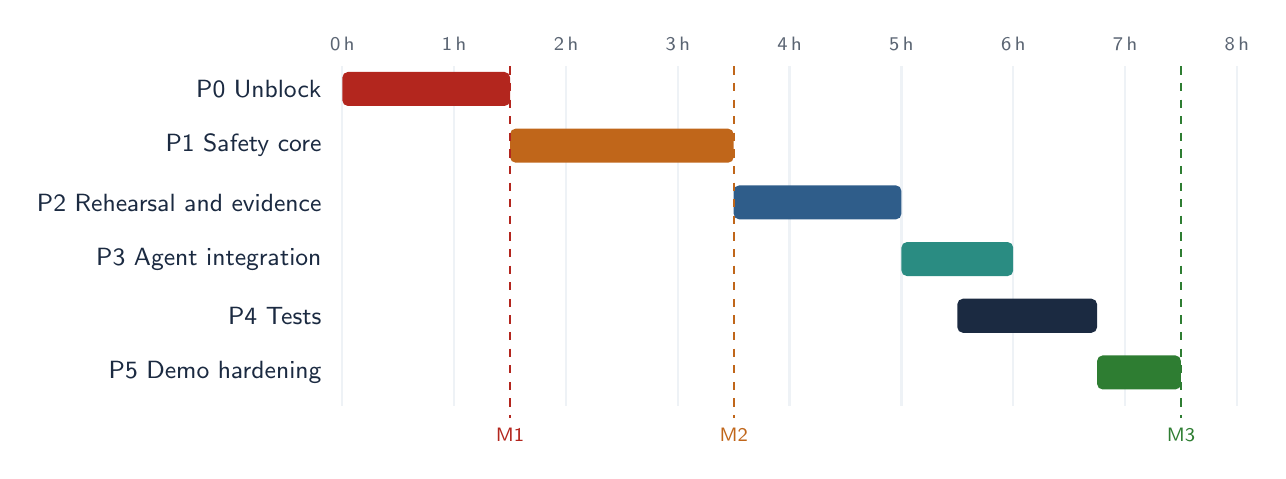
\begin{tikzpicture}[font=\sffamily\small,x=1.42cm,y=0.72cm]
  \foreach \h in {0,...,8} {
    \draw[sflight,thick] (\h,0.4) -- (\h,-5.6);
    \node[text=sfgrey,font=\sffamily\scriptsize] at (\h,0.8) {\h\,h};
  }
  \foreach \y/\name/\s/\e/\c in {
      0/{P0 Unblock}/0/1.5/sfred,
      1/{P1 Safety core}/1.5/3.5/sforange,
      2/{P2 Rehearsal and evidence}/3.5/5/sfblue,
      3/{P3 Agent integration}/5/6/sfteal,
      4/{P4 Tests}/5.5/6.75/sfnavy,
      5/{P5 Demo hardening}/6.75/7.5/sfgreen} {
    \node[anchor=east,text=sfnavy] at (-0.1,-\y) {\name};
    \fill[\c,rounded corners=2pt] (\s,-\y-0.3) rectangle (\e,-\y+0.3);
  }
  \draw[sfred,dashed,thick] (1.5,0.4) -- (1.5,-5.8) node[below,font=\sffamily\scriptsize,text=sfred]{M1};
  \draw[sforange,dashed,thick] (3.5,0.4) -- (3.5,-5.8) node[below,font=\sffamily\scriptsize,text=sforange]{M2};
  \draw[sfgreen,dashed,thick] (7.5,0.4) -- (7.5,-5.8) node[below,font=\sffamily\scriptsize,text=sfgreen]{M3};
\end{tikzpicture}
\end{center}

\begin{tabularx}{\textwidth}{@{}L{1.8cm}L{3.2cm}Y@{}}
\toprule
\sffamily\bfseries Milestone & \sffamily\bfseries Name & \sffamily\bfseries Exit condition \\
\midrule
M1 & Pipeline runs & Phase 0 acceptance met; every tool call succeeds against real databases \\
M2 & Gate enforced & All five token and drift rejection paths are demonstrable \\
M3 & Demo ready & Two clean dry runs, tests green, backup video recorded \\
\bottomrule
\end{tabularx}

% =============================================================================
\section{Five-Minute Demo Run Sheet}
\label{sec:demo}

\begin{longtable}{@{}L{1.9cm}L{3.6cm}L{10.1cm}@{}}
\toprule
\sffamily\bfseries Time & \sffamily\bfseries Beat & \sffamily\bfseries What must be real on screen \\
\midrule
0:00--0:45 & Problem and architecture & Section 3 diagram; point at the red executor boundary \\
0:45--2:00 & Request A & Live \fp{db_inspect_schema} output showing nullable \fp{email} in prod \\
2:00--3:00 & Rehearsal fails & Ephemeral database created; 14 violations with sample ids; packet says DO NOT APPLY; prod fingerprint unchanged \\
3:00--3:40 & Request B & Additive nullable \fp{archived_at}; all checks green \\
3:40--4:20 & Gate & TrueForge frozen; \fp{sf-approve} shows the hash and defaults to reject; human types the hash prefix \\
4:20--5:00 & Execute and verify & Executor applies; \fp{verify_production} confirms; optionally replay the token live to show the rejection \\
\bottomrule
\end{longtable}

% =============================================================================
\section{Risk Register}

\begin{longtable}{@{}L{5.4cm}L{1.9cm}L{8.3cm}@{}}
\toprule
\sffamily\bfseries Risk & \sffamily\bfseries Impact & \sffamily\bfseries Mitigation \\
\midrule
\endhead
TrueForge gate semantics differ from the assumptions in \fp{agent.yaml} & \crit & Validate gate pause and resume in the first hour of Phase 3. Fallback: the executor itself blocks without a token, and the gate only displays the packet \\
SQL parser rejects valid PostgreSQL syntax & \high & Fail closed to REVIEW; keep demo SQL within parser coverage; unit test both demo migrations \\
Template database creation fails while \fp{sf_baseline} has active connections & \med & Never connect tools to the baseline; the refresh script terminates backends first \\
LLM synthesises different SQL across runs & \med & Temperature is already 0.1; the decision depends on rehearsal evidence, not SQL text; the packet shows the hash \\
Secrets committed from \fp{.env} & \high & Confirm \fp{.env} is git-ignored before the first commit; generate the approval secret locally per machine \\
A larger seed slows container start & \low & Keep scale behind a variable; size the demo default to start in under 30 seconds \\
\bottomrule
\end{longtable}

% =============================================================================
\section{Out of Scope}
Following the playbook's scope cuts, these stay out: multi-database support,
Kubernetes, Slack or Jira integration, user authentication, any web UI beyond terminal output,
generic multi-agent orchestration, and automatic rollback of irreversible changes.

% =============================================================================
\appendix
\section{File Change Map}

\begin{longtable}{@{}L{7.4cm}L{1.3cm}L{6.9cm}@{}}
\toprule
\sffamily\bfseries File & \sffamily\bfseries Phase & \sffamily\bfseries Change \\
\midrule
\endhead
\fp{mcp-server/src/config.ts} & 0 & new: zod-validated environment \\
\fp{mcp-server/src/db.ts} & 0 & \fp{withClient}, \fp{withTransaction}; config-driven pools \\
\fp{docker-compose.yml}, \fp{docker/init-*.sql} & 0 & prod loads seed files; \fp{sf_executor} role; ledger schema \\
\fp{shadow/reset-shadow.sh} & 0 & correct credentials \\
\fp{.env.example}, \fp{README.md} & 0 & align names, paths and transport \\
\fp{mcp-server/src/safety/classifier.ts} & 1 & new \\
\fp{mcp-server/src/safety/approval.ts} & 1 & new: sign, verify, canonical JSON \\
\fp{mcp-server/src/executor.ts} & 1 & new entry point hosting \fp{execute_migration} \\
\fp{mcp-server/src/tools/execute_migration.ts} & 1 & signature, ledger, drift check, execution modes \\
\fp{mcp-server/src/index.ts} & 1 & remove executor tool; refuse a write URL \\
\fp{shadow/refresh-baseline.sh} & 2 & new: dump prod into \fp{sf_baseline} \\
\fp{mcp-server/src/tools/rehearse_migration.ts} & 2 & ephemeral template database; invariants; rollback \\
\fp{mcp-server/src/verification/*} & 2 & moved from \fp{verification/} \\
\fp{mcp-server/src/tools/build_decision_packet.ts} & 2 & new: rule engine \\
\fp{mcp-server/src/tools/verify_production.ts} & 2 & identifier validation \\
\fp{mcp-server/src/tools/readonly_query.ts} & 2 & \texttt{BEGIN READ ONLY} \\
\fp{trueforge-config/agent.yaml}, \fp{system-prompt.md} & 3 & two servers, gate, tool order \\
\fp{mcp-server/src/cli/approve.ts} & 3 & new: human-side signer \\
\fp{mcp-server/test/} & 4 & new: T1--T12 \\
\fp{scripts/demo-reset.sh} & 5 & new \\
\bottomrule
\end{longtable}

\end{document}
